% !TEX program = xelatex
\documentclass[tikz,border=0pt]{standalone}
\usepackage{fontspec}
\usepackage{xcolor}
\usetikzlibrary{calc,shapes.geometric}

% Las fuentes se cargan directamente desde la carpeta "fonts" que va junto a
% este .tex (no hace falta instalarlas en Windows). Si mueves el .tex,
% mueve la carpeta "fonts" con él.
\setmainfont{Cinzel-Variable}[Path=./fonts/,Extension=.ttf]
\newfontfamily\cinzeldec{CinzelDecorative-Bold}[Path=./fonts/,Extension=.ttf]
\newfontfamily\cinzel{Cinzel-Variable}[Path=./fonts/,Extension=.ttf]
\newfontfamily\medieval{MedievalSharp}[Path=./fonts/,Extension=.ttf]

\definecolor{bgdeep}{HTML}{150C22}
\definecolor{bgmid}{HTML}{271A3D}
\definecolor{bgvign}{HTML}{0B0714}
\definecolor{violetmid}{HTML}{4A2E6B}
\definecolor{violetglow}{HTML}{8E5FC2}
\definecolor{violetsoft}{HTML}{B58EDB}
\definecolor{silver}{HTML}{C9CDE0}
\definecolor{silverbright}{HTML}{F1F2F8}
\definecolor{silverdim}{HTML}{8D89A3}

\begin{document}
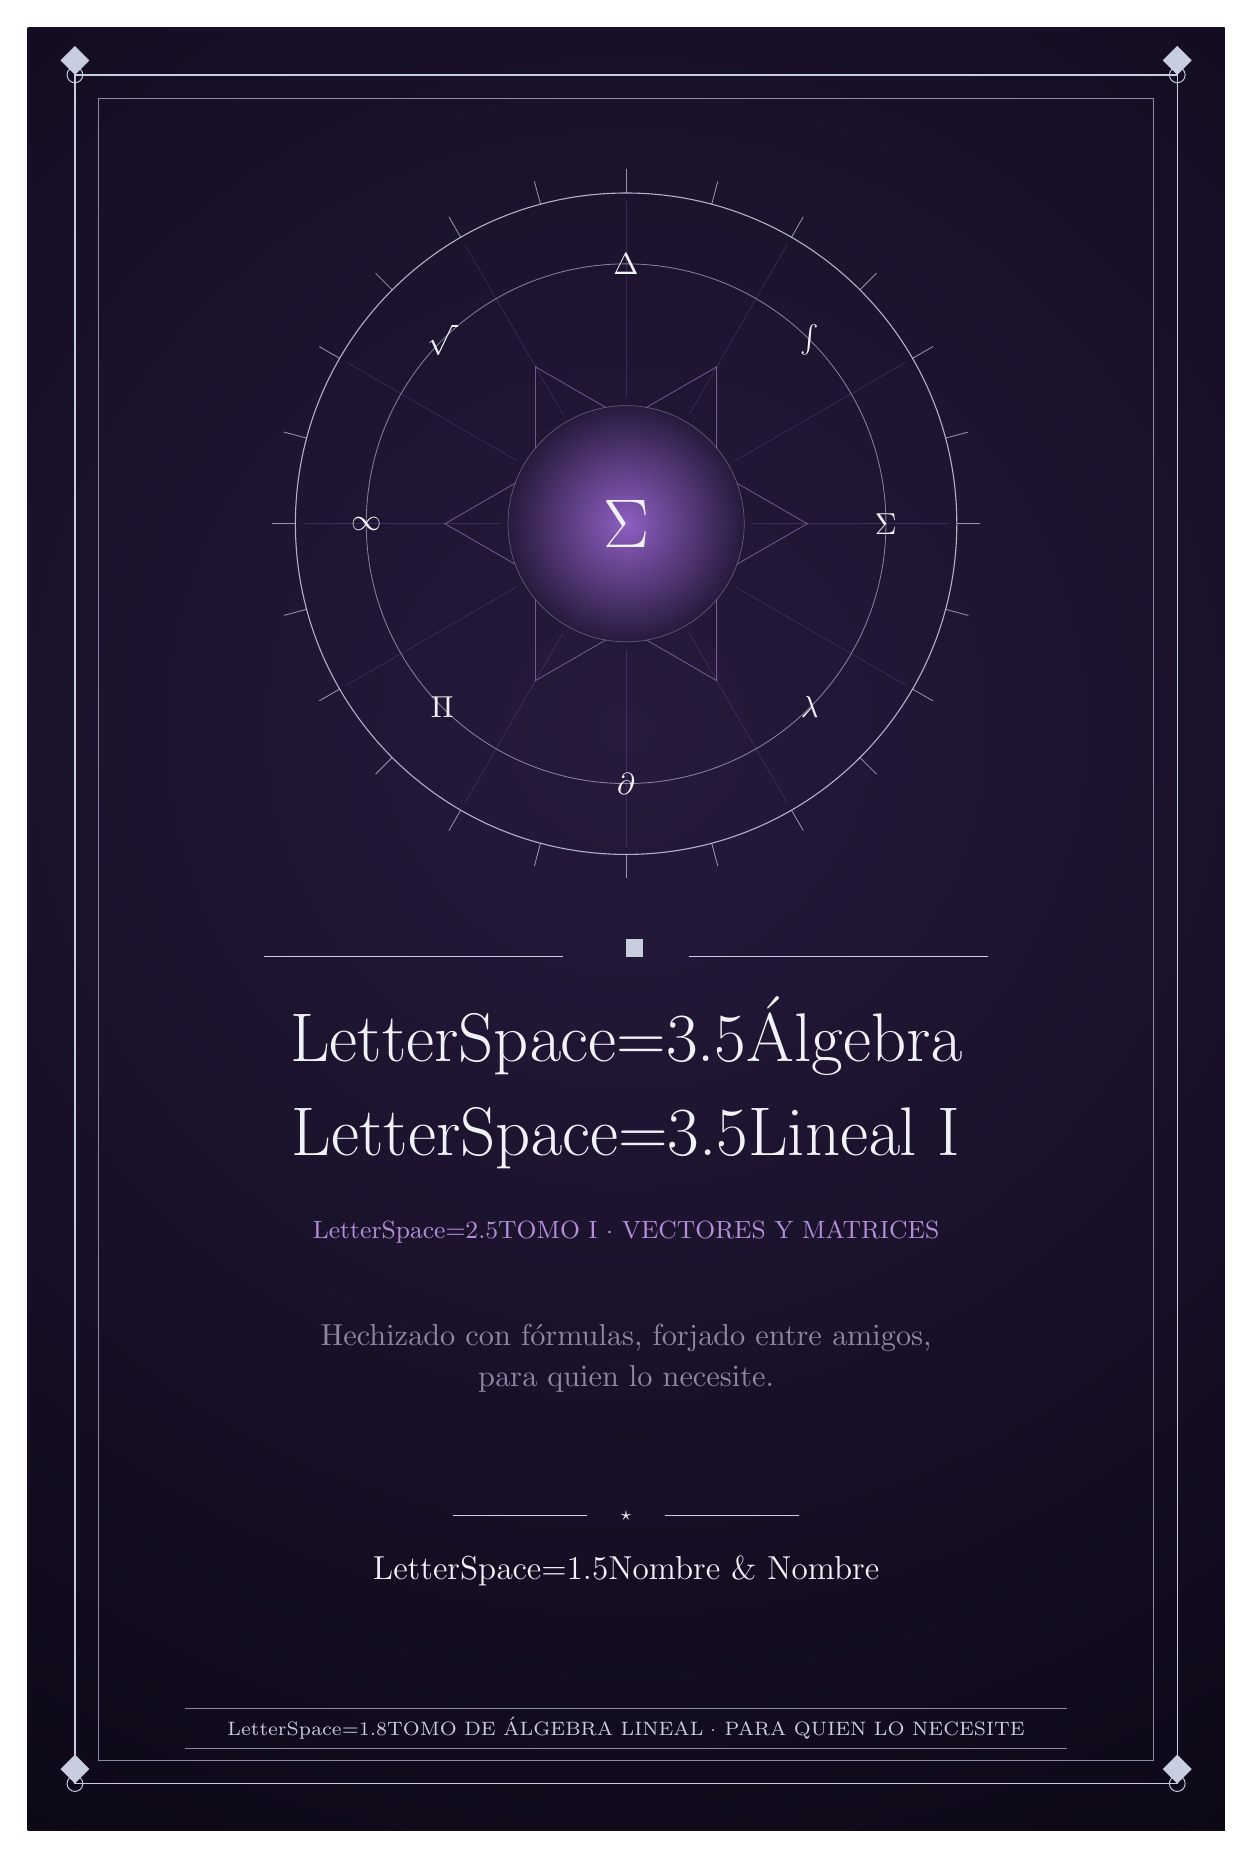
\begin{tikzpicture}[x=1mm,y=1mm]

  % ===================== BACKGROUND ======================
  \fill[bgvign] (0,0) rectangle (152,229);
  \begin{scope}
    \clip (0,0) rectangle (152,229);
    \shade[shading=radial,inner color=bgmid,outer color=bgvign] (76,140) circle (170mm);
  \end{scope}

  % ===================== ORNATE FRAME ======================
  \draw[silver,line width=0.55] (6,6) rectangle (146,223);
  \draw[silverdim,line width=0.22] (9,9) rectangle (143,220);

  % corner ornaments
  \foreach \cx/\cy in {6/223,146/223,6/6,146/6}{
    \begin{scope}[shift={(\cx,\cy)}]
      \fill[silver] (0,0) ++(45:2.6) -- ++(135:2.6) -- ++(225:2.6) -- ++(315:2.6) -- cycle;
      \draw[silver,line width=0.35] (0,0) circle (1.0mm);
    \end{scope}
  }

  % ===================== MAGIC CIRCLE ======================
  \coordinate (C) at (76,166);

  % faint radial spokes
  \foreach \ang in {0,30,...,330}{
    \draw[violetglow,opacity=0.28,line width=0.25] ($(C)+(\ang:16)$) -- ($(C)+(\ang:41)$);
  }

  % outer ring + ticks
  \draw[silver,opacity=0.85,line width=0.4] (C) circle (42mm);
  \foreach \ang in {0,15,...,345}{
    \draw[silver,opacity=0.7,line width=0.3] ($(C)+(\ang:42)$) -- ($(C)+(\ang:45)$);
  }

  % middle ring with algebra "runes"
  \draw[silver,opacity=0.6,line width=0.3] (C) circle (33mm);
  \foreach \ang/\sym in {0/{\Sigma},45/{\int},90/{\Delta},135/{\sqrt{\,}},
                          180/{\infty},225/{\Pi},270/{\partial},315/{\lambda}}{
    \node[silverbright,font=\fontsize{11}{11}\selectfont] at ($(C)+(\ang:33)$) {$\sym$};
  }

  % hexagram
  \foreach \rot in {0,60}{
    \draw[violetsoft,opacity=0.55,line width=0.3]
      ($(C)+(\rot+0:23)$) -- ($(C)+(\rot+120:23)$) -- ($(C)+(\rot+240:23)$) -- cycle;
  }

  % inner glow + centerpiece
  \shade[shading=radial,inner color=violetglow,outer color=bgmid] (C) circle (15mm);
  \draw[silverdim,opacity=0.6,line width=0.25] (C) circle (15mm);
  \node[silverbright,font=\fontsize{40}{40}\selectfont] at (C) {$\Sigma$};

  % ===================== DIVIDER ======================
  \draw[silver,line width=0.35] (30,111) -- (68,111);
  \draw[silver,line width=0.35] (84,111) -- (122,111);
  \begin{scope}[shift={(76,111)}]
    \fill[silver] (0,0) ++(0:2.2) -- ++(90:2.2) -- ++(180:2.2) -- ++(270:2.2) -- cycle;
  \end{scope}

  % ===================== TITLE ======================
  \node[text=silverbright,font=\cinzeldec\fontsize{30}{34}\selectfont]
    at (76,101) {\addfontfeature{LetterSpace=3.5}Álgebra};
  \node[text=silverbright,font=\cinzeldec\fontsize{30}{34}\selectfont]
    at (76,88) {\addfontfeature{LetterSpace=3.5}Lineal I};

  % subtitle
  \node[text=violetsoft,font=\cinzel\fontsize{9.5}{12}\selectfont]
    at (76,76) {\addfontfeature{LetterSpace=2.5}TOMO I \textperiodcentered\ VECTORES Y MATRICES};

  % tagline
  \node[text=silverdim,align=center,text width=112mm,
        font=\medieval\fontsize{11}{15}\selectfont]
    at (76,60) {Hechizado con fórmulas, forjado entre amigos,\\ para quien lo necesite.};

  % byline ornament
  \begin{scope}[shift={(76,40)}]
    \draw[silver,line width=0.3] (-22,0) -- (-5,0);
    \draw[silver,line width=0.3] (5,0) -- (22,0);
    \node[silverbright,font=\fontsize{7}{7}\selectfont] at (0,0) {$\star$};
  \end{scope}
  \node[text=silverbright,font=\cinzel\fontsize{12}{14}\selectfont]
    at (76,33) {\addfontfeature{LetterSpace=1.5}Nombre \& Nombre};

  % ===================== FOOTER NAMEPLATE ======================
  \draw[silverdim,line width=0.22] (20,15.5) -- (132,15.5);
  \draw[silverdim,line width=0.22] (20,10.5) -- (132,10.5);
  \node[text=silver,font=\cinzel\fontsize{7}{8}\selectfont]
    at (76,13) {\addfontfeature{LetterSpace=1.8}TOMO DE ÁLGEBRA LINEAL \textperiodcentered\ PARA QUIEN LO NECESITE};

\end{tikzpicture}
\end{document}
